\section{Sequential}

\frame{\frametitle{Index}\tableofcontents[currentsection,subsectionstyle=show/show/shaded]}

\subsection{Original}
\begin{frame}
	\frametitle{Original implementation}
	\begin{itemize}
		\item \textbf{\itshape Arrays-of-Pointers};
		\item Prepared for \textbf{dynamic cell velocities}\ \textit{(not implemented)};
		\item Animated simulation;
	\end{itemize}

	\begin{columns}
		\column{.45\textwidth}
		\pause
		\begin{block}{\computeflux}
			\smaller
			For all \textbf{edges}:
			\begin{enumerate}
				\item Read adjacent cell data;	
				\item Compute edge velocity;
				\item Compute flux through edge;
				\item Compute $v_{max}$ and $\Delta t$;
			\end{enumerate}
		\end{block}

		\column{.45\textwidth}
		\pause
		\begin{block}{\update}
			\smaller
			For all \textbf{edges}:
			\begin{enumerate}
				\item Subtract flux from left cell;
				\item Add flux to right cell;
			\end{enumerate}
		\end{block}
	\end{columns}
\end{frame}

\subsection{Optimizations}
\begin{frame}
	\frametitle{Optimizations}
	\begin{columns}
		\smaller
		\column{0.4\textwidth}
			\centering
			\textbf{\itshape Array-Of-Structs}

			\smaller
			\begin{tabular}{|c|c|}
				\hline
				\multirow{4}{*}{$S_{1}$} & $e_{1}$\\
				\cline{2-2}
				& $e_{2}$\\
				\cline{2-2}
				& $e_{3}$\\
				\cline{2-2}
				& \ldots\\
				\hline
				\multirow{4}{*}{$S_{2}$} & $e_{1}$\\
				\cline{2-2}
				& $e_{2}$\\
				\cline{2-2}
				& $e_{3}$\\
				\cline{2-2}
				& \ldots\\

				\hline
				\multirow{5}{*}{$S_{3}$} & $e_{1}$\\
				\cline{2-2}
				& $e_{2}$\\
				\cline{2-2}
				& $e_{3}$\\
				\cline{2-2}
				& \dots\\
				\hline
				\multicolumn{2}{|c|}{\ldots}
			\end{tabular}
			\larger

			\begin{itemize}
				\item Pointers $\Rightarrow$ Indexes;
			\end{itemize}

		\column{0.4\textwidth}
			\pause
			\centering
			\textbf{\itshape Structs-Of-Arrays}

			\smaller
			\begin{table}
				\captionsetup[subfloat]{position=top,labelformat=empty}
				\subfloat[$e_{1}$]{%
				\begin{tabular}{|c|}
					\hline
					$S_{1}$\\
					\hline
					$S_{2}$\\
					\hline
					$S_{3}$\\
					\hline
					\ldots
				\end{tabular}%
				}\;
				\subfloat[$e_{2}$]{%
				\begin{tabular}{|c|}
					\hline
					$S_{1}$\\
					\hline
					$S_{2}$\\
					\hline
					$S_{3}$\\
					\hline
					\ldots
				\end{tabular}%
				}\;
				\subfloat[$e_{3}$]{%
				\begin{tabular}{|c|}
					\hline
					$S_{1}$\\
					\hline
					$S_{2}$\\
					\hline
					$S_{3}$\\
					\hline
					\ldots
				\end{tabular}%
				}\;
				\subfloat[\ldots]{}
			\end{table}
			\larger

			\begin{itemize}
				\item Pointers $\Rightarrow$ Indexes;
				\item Loads only what is needed;
			\end{itemize}
	\end{columns}
\end{frame}


\begin{frame}
	\frametitle{Results}
	\begin{figure}
		\centering
		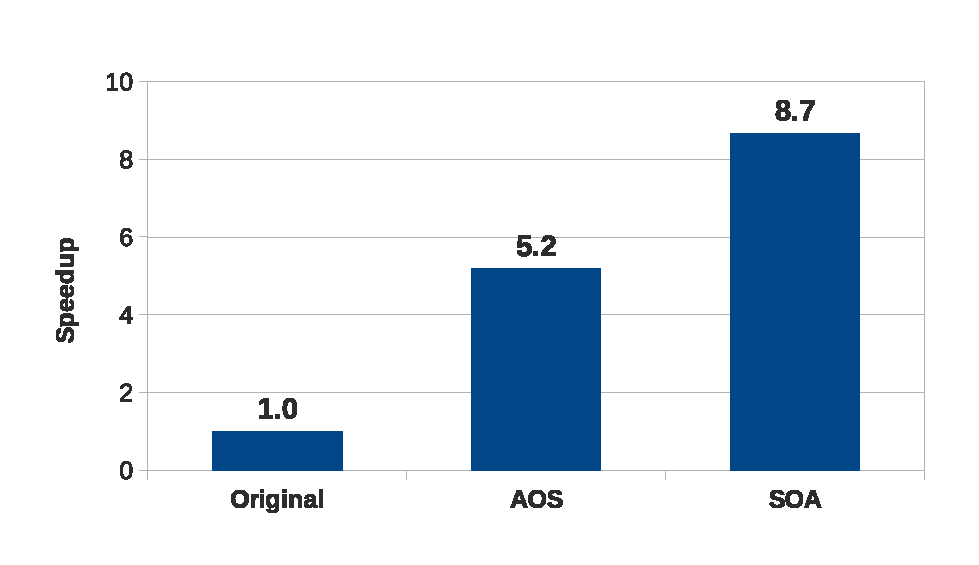
\includegraphics[width=0.8\textwidth]{graph_comparison_seq.eps}
	\end{figure}
\end{frame}


\subsection{Dependencies}
\begin{frame}
	\frametitle{Dependencies}
	\begin{block}{\computeflux}
		\begin{columns}
			\column{0.45\textwidth}
				\begin{itemize}
					\item $\Delta t$ requires $\mathrm{max}(v)$;
				\end{itemize}

			\column{0.05\textwidth}
				\larger
				$\Rightarrow$

			\column{0.45\textwidth}
				\begin{itemize}
					\item [+] Reduction;
					\item [+] Cell velocities are \textbf{constant};
				\end{itemize}
		\end{columns}
	\end{block}
	\pause
	\begin{block}{\update}
		\begin{columns}
			\column{0.45\textwidth}
				\begin{itemize}
					\item Race condition;
				\end{itemize}
				\begin{figure}
					\centering
					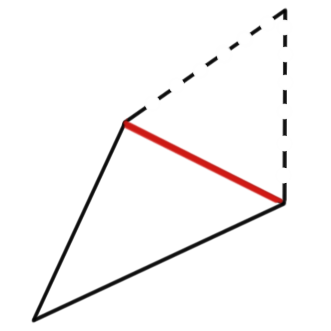
\includegraphics[width=.5\textwidth]{edge.png}
				\end{figure}

			\column{0.05\textwidth}
				\larger
				$\Rightarrow$

			\column{0.45\textwidth}
				\begin{itemize}
					\item [+] Iterate over cells;
				\end{itemize}
				\begin{figure}
					\centering
					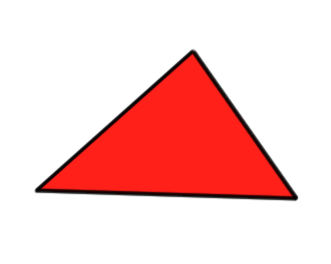
\includegraphics[width=.7\textwidth]{cell.png}
				\end{figure}
		\end{columns}
	\end{block}
\end{frame}
